\section{Aufbau}

\begin{minipage}{0.5\textwidth}
Maßgebend für den Aufbau ist der $50 \si{\liter}$ große, mit Edelstahl umhüllte Szintillator vom Typ \enquote{NE 102} und mit Tuluol gefüllt. Diesem ist ein eigener Abschnitt gewidmet und dort entsprechend erläutert. \ref{kommt}
Mit ihm werden die einfallenden Myonen für die Detektion sichtbar gemacht. Da die entstehenden Signale schwach sind, bietet es sich an diese durch einen Sekundärelektronenverstärker, kurz SEV zu verstärken. An diesen Verstärkern ist für
die Funnktionalität eine Hochspannung angelegt. Dieser Teil des Aufbaus ist symetrisch an beiden Stirnseiten des Szintillator angebracht. So ist es also möglich die einfallenden Teilchen als Lichtsignal durch die SEV auszulesen.
Das Signal der zwei Sekundärelektronenverstärker kann durch vielerlei Gründe einseitig verschoben sein, das heißt es tritt durch asymetrische Verzögerungen eine zeitliche Differenz $\increment t$ auf.
\end{minipage}
Der Zeitlichen Differenz zwischen den SEVs kann man durch passend eingesetzte \enquote{Delays} entgegenwirken. Diese sind weiter Kabel, die durch ihre whählbare Länge die Zeit verzögern. 
\begin{figure}
    \centering
    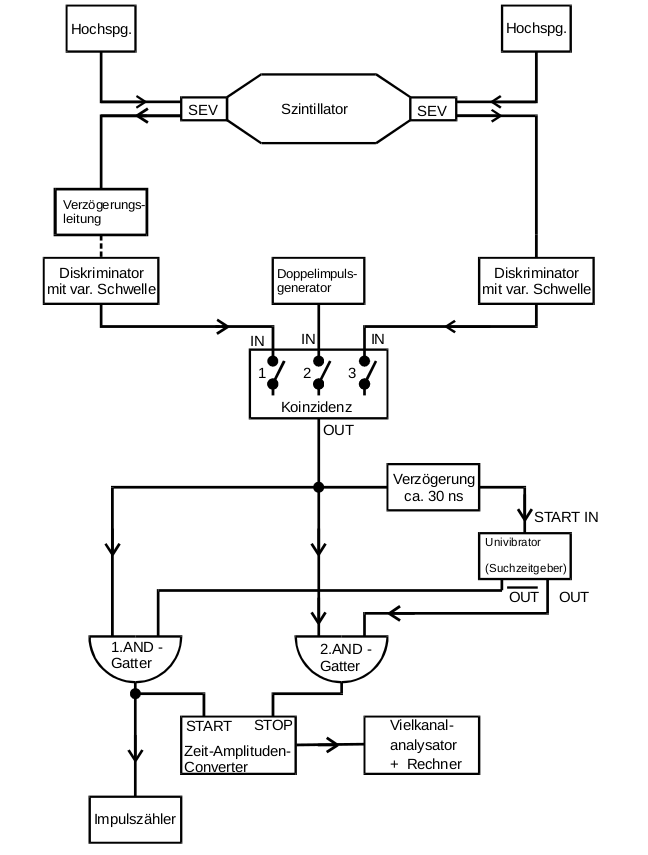
\includegraphics[width=0.6\textwidth]{bilder/aufbau.png}
    \caption{Schematischer Aufbau zur bestimmung der Lebensdauer von Myonen. \cite{skript}} 
    \label{fig:1}
\end{figure}